%	Auteur: Surdez Quentin
%	Titre:	 Étudiant MCT
%	Date: Mai 2022
%	Sujet: Rapport de projet P2213	
%============================================================
\documentclass[
	a4paper,									% paper format
	11pt,										% fontsize
	twoside,									% double-sided
	openright,									% begin new chapter on right side
	notitlepage,									% use no standard title page
	parskip=half,								% set paragraph skip to half of a line
]{scrreprt}										% KOMA-script report
%---------------------------------------------------------------------------

\raggedbottom
\KOMAoptions{cleardoublepage=plain}						%Add header and footer on blank pages

%Load Standard Packages: 
%---------------------------------------------------------------------------
\usepackage[standard-baselineskips]{cmbright}				%Fonts for math equation
\usepackage[french]{babel}							%French hyphenation
	%\usepackage[latin1]{inputenc}  					% Unix/Linux - load extended character set (ISO 8859-1)
	%\usepackage[applemac]{inputenc}
	%\usepackage[ansinew]{inputenc}  					% Windows - load extended character set (ISO 8859-1)
%\usepackage[utf8]{inputenc}							%Translate input in latex language
\usepackage[T1]{fontenc}							%Allow a good hyphenation with accentuated language
%\usepackage{tgbonum}
\usepackage{ae}									%Allow vectorial letters
\usepackage{lmodern}
\usepackage{fancyhdr}								%Allow manipulation on headers and tops
\usepackage{graphicx}								%Integration of images
\usepackage{float}									%Better integration of floating objects(tables, etc)
\usepackage{caption}								%For captions of figures and tables
\usepackage{booktabs}								%Nicer tables
\usepackage{tocvsec2}								%Means of controlling the sectional numbering
\usepackage{verbatim}								%Integration of source code
\usepackage{moreverb}								%Extension of verbatim
\usepackage{listings}								%Integration of code in LATEX 
\usepackage{multirow}								%Tables with multiple rows
\usepackage{pdfpages}						
\usepackage{pst-all}								%Better handling of texts and images
\usepackage{mathrsfs}
\usepackage{colortbl}
\usepackage{listings}
\usepackage{minted}								%Better colorizing of source code WARNING need to be set up correctly according to the documentation http://tug.ctan.org/macros/latex/contrib/minted/minted.pdf
\usepackage{ragged2e}
\captionsetup{font=small}
\usepackage{siunitx}
\usepackage{wrapfig}
\sisetup{
    round-mode      = places, %Round numbers
    round-precision = 2, % to 2 places
}

\usepackage{booktabs}


\newcolumntype{R}[1]{>{\raggedleft\arraybackslash }b{#1}}
\newcolumntype{L}[1]{>{\raggedright\arraybackslash }b{#1}}
\newcolumntype{C}[1]{>{\centering\arraybackslash }b{#1}}		%Adding new column types

%---------------------------------------------------------------------------

%Load Math packages
%---------------------------------------------------------------------------
\usepackage{amsmath}                    				   	% various features to facilitate writing math formulas
\usepackage{amsthm}                       	 				% enhanced version of latex's newtheorem
\usepackage{amsfonts}                      					% set of miscellaneous TeX fonts that augment the standard CM
										
\usepackage{amssymb}							% mathematical special characters
\usepackage{exscale}							% mathematical size corresponds to textsize
\usepackage{listings}
\usepackage{tikz,pgfplots}
\usepackage{array}
%---------------------------------------------------------------------------

%QR Code
%---------------------------------------------------------------------------
\usepackage{qrcode}
\usepackage{subcaption}							%Add sub-caption easily
%---------------------------------------------------------------------------

% Package to facilitate placement of boxes at absolute positions
%---------------------------------------------------------------------------
%\usepackage[absolute]{textpos}
\usepackage[absolute,overlay]{textpos}
\setlength{\TPHorizModule}{1mm}
\setlength{\TPVertModule}{1mm}
%---------------------------------------------------------------------------	

% Definition of Colors
%---------------------------------------------------------------------------
\RequirePackage{color}							% Color (not xcolor!)
\definecolor{linkblue}{rgb}{0,0,0.8}            				% Standard
\definecolor{darkblue}{rgb}{0,0.08,0.45} 				% Dark blue
\definecolor{brickred}{cmyk}{0,0.89,0.94,0.28} 			% Brickred
\definecolor{linkcolor}{rgb}{0,0,0}        					% Black for the print-version!
\definecolor{PEjaune}{rgb}{1,0.84,0}        				% Jaune PE
\definecolor{PEvert}{rgb}{0.14,0.5,0}        				% Vert PE

\definecolor{VertVAUD}{rgb}{0.054, 0.662, 0.301} %14, 169, 77}

%---------------------------------------------------------------------------

% Hyperref Package (Create links in a pdf)
%---------------------------------------------------------------------------
\usepackage[
	pdftex,frenchb,bookmarks,plainpages=false,pdfpagelabels,
	backref = {false},							% No index backreference
	colorlinks = {true},							% Color links in a PDF
	hypertexnames = {true},						% no failures "same page(i)"
	bookmarksopen = {true},						% opens the bar on the left side
	bookmarksopenlevel = {0},					% depth of opened bookmarks
	pdftitle = {Rapport Projet P2213},		   		% PDF-property
	pdfauthor = {Surdez Quentin},        				% PDF-property
	pdfsubject = {Promotion 21-22},        				% PDF-property
	linkcolor = {linkcolor},              					% Color of Links
	citecolor = {linkcolor},              					% Color of Cite-Links
	urlcolor = {linkblue},               					% Color of URLs
]{hyperref}
%---------------------------------------------------------------------------

% Set up page dimension
%---------------------------------------------------------------------------
\usepackage[
	a4paper,
	left=30mm,
	right=30mm,
	top=30mm,
	headheight=20mm,
	headsep=10mm,
	textheight=242mm,
	footskip=15mm
]{geometry}
\setlength\parindent{20pt}
%---------------------------------------------------------------------------

% Makeindex Package
%---------------------------------------------------------------------------
\usepackage{makeidx}                         					% To produce index
\makeindex                                    					% Index-Initialisation
%---------------------------------------------------------------------------

% Intro:
\pgfplotsset{compat=1.18} 
%---------------------------------------------------------------------------
\begin{document}                              					% Start Document
\settocdepth{subsection}									% Set depth of toc
\pagenumbering{roman}														
%---------------------------------------------------------------------------

%Set up header and footer
%---------------------------------------------------------------------------
\fancyhf{}												%clean all fields
\fancypagestyle{plain}{									%new definition of plain style
	\fancyfoot[OR, EL]{\footnotesize \thepage}			%footer right part --> page number
	\fancyfoot[OL, ER]{\footnotesize \leftmark}			%footer left part --> chapter
	\fancyfoot[CE, CO]{P2213, QS \& RD}
	\fancyhead[C]{
	\begin{textblock}{0}[0, 0](10, 8)						%header center part --> logo CPNV + MCT 
		
\includegraphics[scale=0.7]{img/logoCPNV.png}
	\end{textblock}
	\begin{textblock}{0}[0, 0](175, 3)
		\includegraphics[scale=0.5]{img/logoMCT.jpg}
	\end{textblock}
	}
}

\renewcommand{\chaptermark}[1]{\markboth{\thechapter.  #1}{}}
\renewcommand{\headrulewidth}{0pt}				% no header stripline
\renewcommand{\footrulewidth}{0pt} 				% no bottom stripline

\pagestyle{plain}
\let\cleardoublepage\clearpage
%---------------------------------------------------------------------------

%=============================================================================================
% Page principale
%=============================================================================================
%---------------------------------------------------------------------------
\begin{titlepage}
	\setlength{\unitlength}{1mm}
%	\begin{textblock}{230}(-10,-10)
%		\begin{picture}(230,35)%32)
%			\put(73,0){\color{VertVAUD}\rule{160mm}{40mm}}
%		\end{picture}
%	\end{textblock}

	\begin{textblock}{0}[0,0](5,12) % (x,y)
		
\includegraphics[scale=1]{img/logoCPNV.png}
	\end{textblock}

	\begin{textblock}{0}(158, 2)
		\includegraphics[scale=0.8]{img/logoMCT.jpg}
	\end{textblock}





% Titre / Sous-titre / Auteur / Image de garde:
%---------------------------------------------------------------------------
	
	\flushleft
	\vspace*{1cm}
	%\fontfamily{cmr}\selectfont			%To have the default font
	\fontsize{18pt}{20pt}\selectfont
	CPNV - Centre Professionnel du Nord Vaudois \\
	\fontsize{12pt}{15pt}\selectfont\vspace{0.5em}
	MCT - Modules complémentaires techniqeus

	\vspace{3cm}

	\fontsize{30pt}{32pt}\selectfont 
	\noindent \textbf{Communication externe} \\

	\fontsize{18pt}{20pt}\selectfont\vspace{0.3em} P2213 \\

	\vspace{4cm}
	\fontsize{12pt}{15pt}\selectfont
	\begin{tabbing}
		xxxxxxxxxxxxxxx\=xxxxxxxxxxxxxxxxxxxxxxx \kill
		Rédacteur:\> Quentin Surdez\\ \\
		Relecture:\> Rafael Dousse\\ \\
		École:\> CPNV\\ \\
		Date:\> Yverdon-Les-Bains, le \today \\
	\end{tabbing}
\end{titlepage}
%---------------------------------------------------------------------------

%===========================================
% Table des matières
%===========================================
\tableofcontents

\listoffigures									% Table des figures
\listoftables									% Table des tableaux
\cleardoublepage
%---------------------------------------------------------------------------

%=============================================================================================
% Introduction
%=============================================================================================
\pagenumbering{arabic}
\setcounter{page}{1}

\chapter{Introduction}
Ce document a pour but d'expliquer notre construction de la communication externe du robot. 
La communication externe se compose du Raspberry PI, de l'Arduino Nano ainsi que d'un 
objet connecté via un réseau WIFI à notre Raspberry PI. Nous discuterons de nos approches pour utiliser la communication
et de comment nous avons résolu les différents problèmes que nous avons rencontrés. 

%=============================================================================================
% Document
%=============================================================================================
\chapter{Serveur}

Nous avons recherché à faire de notre Raspberry PI un serveur permettant d'héberger une web application.
Cela permettrait à notre application d'être facilement accessible tant que le Raspberry PI est connecté au même réseau
WIFI que l'appareil qui servira de contrôle pour le robot. \par

\section{Apache}

\begin{figure}[!ht]
	\centering
	
\includegraphics[scale=.1]{img/Apache.png}
	\label{Apache}
	\caption{Logo du serveur Web Apache}
\end{figure}

Apache est la première alternative que nous avons essayé. C'est un serveur Web HTTP qui aurait permis d'héberger notre web
application. Nous l'avons peu à peu pris en main et nous avons réussi à utiliser le Raspberry en hotspot. Cependant, Apache 
restait relativement obscure pour nous. Les différentes possibilités qu'Apache offrait ne correspondait pas à nos besoins. 
Nous ne souhaitions pas héberger sur le web une application, nous ne souhaitions pas faire de notre Raspberry PI un serveur. \par

\section{ROS}

Nous avons eu une autre alternative pour faire de notre Raspberry PI hotspot. Le système d'exploitation ROS, pour Robotic Operating System, 
nous offrait cette possibilité, tout en étant pensé et developpé pour des robots. Nous avons pris connaissance des possibilités 
que cet OS offrait, comme la création de noeud de communications. Cependant, nous avons vite compris que ROS était principalement
fait pour des robots industriels ou de qualité supérieure au notre. Après plusieurs tentatives, nous n'avons pas réussi à installer 
l'OS sur notre Raspberry PI. Nous nous sommes éloignés de l'idée de paramétré notre Raspberry PI en hotspot. \par

\newpage
\section{Flask}

\begin{figure}[!ht]
	\centering
	
\includegraphics[scale=.2]{img/Flask.png}
	\vspace{.5cm}
	\label{Flask}
	\captionabove{Logo du micro-framework Flask}
\end{figure}

Nous avons découvert Flask via un tutoriel \href{https://pyimagesearch.com/2019/09/02/opencv-stream-video-to-web-browser-html-page/}{pyimagesearch.com}
la possibilité d'utiliser le micro-framework Flask pour facilement intéragir avec une web application via notre script Python.
Un framework est un logiciel facilitant l'intéraction avec un utilisateur, donc facilitant la création d'applications. 
Flask est un micro-framework car il ne nécessite aucune librairies ou fichier additionnel pour fonctionner. Des extensions
existent pour, par exemple, lui ajouter une fonctionnalité de database avec SQLAlchemy. \par

Ainsi, Flask nous a permis de communiquer avec une page web et de communiquer l'information donnée sur cette page 
à notre script Pyhton. L'information récupérée peut être utilisée dans notre programme. 
Ce protocole est celui que nous avons choisi pour notre communication externe. Nous pouvons nous intéresser de plus 
près sur la strucutre de notre web app. \par

\section{Tableau récapitulatif}

\begin{table}[h!]
    \begin{center}
        \caption{Comparaison des différentes solutions échelle 1 à 10 (1 le moins bon, 10 le meilleur)}
        \vspace{5mm}
        \label{tab:table1}
        \begin{tabular}{c|l|c|r} % <-- Alignments: 1st column left, 2nd middle and 3rd right, with vertical lines in between
            \toprule
            \textbf{ } & \textbf{Apache} & \textbf{ROS} & \textbf{Flask}\\
            Installation & 10 & 1 & 10 \\
            Facilité de prise en main & 5 & 1 & 8\\
            Compatibilité & ? & ? & 10\\
			\midrule
			Total & 15 & \cellcolor{red}{2} & \cellcolor{green}{28}\\
            \bottomrule
        \end{tabular}
    \end{center}    
\end{table}

Ci-dessus, les critères utilisés pour choisir ce avec quoi construire notre communication externe. 
Le choix s'est fait après avoir réussi un à utiliser OpenCV et Flask facilement l'un avec l'autre. 
La compatibilité avec OpenCV d'Apache et ROS n'a pas été testé. \par


\chapter{Web Application}

Nous avons pu nous lancer dans la conception de notre Web Application. Sa structure sera détaillée dans la section suivante. 
Nous avons utilisé HTML/CSS pour pouvoir construire l'architecture du site hébergé sur le Raspberry PI. \par

\section{Structure}

\begin{figure}[!ht]
	\centering
	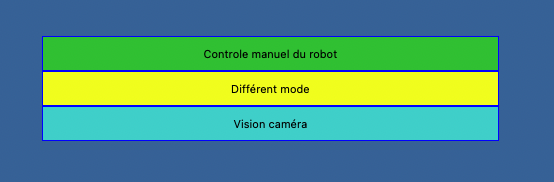
\includegraphics[scale=.5]{img/Page_Accueil_texte.png}
	\vspace{.5cm}
	\label{Accueil}
	\captionabove{Page d'accueil}
\end{figure}

La page d'accueil possède un menu nous permettant de naviguer dans notre site. Nous avons troix choix à notre diposition. 
\begin{itemize}
 \item Le premier "Controle manuel du robot" nous permet d'accéder à la page de contrôle à distance du robot. 
 \item Le second "Différent mode" renvoit sur la page de choix pour les modes de notre robot. 
 \item Le dernier "Vision Caméra" permet d'accéder à une page ayant un stream direct de la caméra du robot.
\end{itemize}

\newpage


\begin{figure}[!ht]
	\centering
	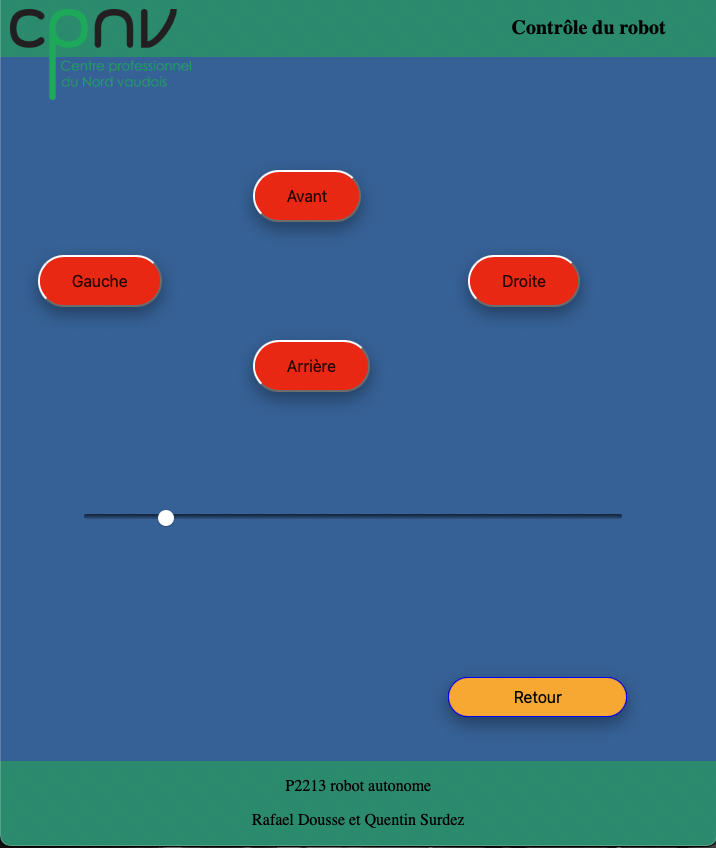
\includegraphics[scale=.5]{img/Controle_Robot.png}
	\vspace{.5cm}
	\label{Controle}
	\captionabove{Page de contrôle du robot}
\end{figure}

La page de Contrôle du robot possède 4 boutons disposés en étoiles. Ces boutons permettent 
d'envoyer des ordres au robot pour se diriger dans les quatre directions d'un plan. Une barre 
latérale ou verticale selon si vous êtes sur un smartphone ou un ordinateur, permet de contrôler 
la vitesse du robot. Nous ne savons si elle restera dans l'implémentation finale. Un bouton "Retour"
permet de revenir à la page d'accueil. \par

\newpage

\begin{figure}[!ht]
	\centering
	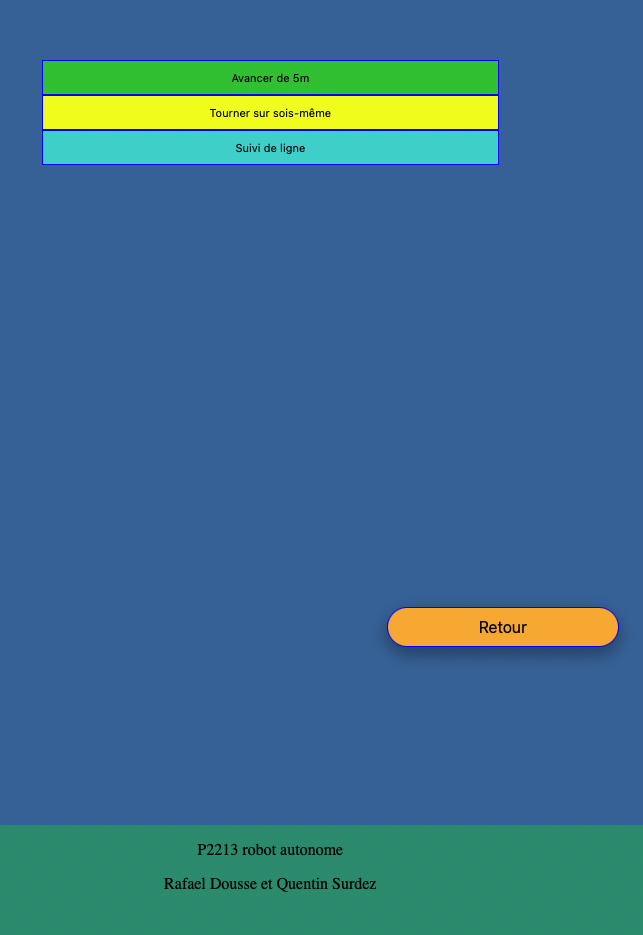
\includegraphics[scale=.4]{img/Choix_Mode_mini.png}
	\vspace{.5cm}
	\label{Choix}
	\captionabove{Page de choix des modes}
\end{figure}

La page de choix de mode du robot possède 3 boutons. Ces boutons permettent d'envoyer des ordres pour excéuter les différents modes du robot.

\begin{itemize}
	\item Le premier "Avancer de 5m" fait avancer le robot de 5m tout droit. 
	\item Le second "Tourner sur soi-même" fait faire un tour au robot sur lui-même.
	\item Le dernier "Suivi de ligne" fait suivre une ligne au robot. 
\end{itemize}

\chapter{Conclusion}

Nous avons pu tester plusieurs méthodes pour accéder à l'hébergement d'une web app sur un Raspberry PI. 
L'outil nous permettant le plus de possibilité est Flask. \par
Grâce à cet outil, nous avons pu facilement communiquer entre la page Web et notre Raspberry PI. 




\end{document}